\documentclass[12pt,a4paper]{article}
\usepackage{charter}
\usepackage[utf8]{inputenc}
%\usepackage[latin1]{inputenc}
\usepackage[left=1.50cm, right=1.50cm, top=1.20cm]{geometry}
\usepackage{amsmath}
\usepackage{amsfonts}
\usepackage{amssymb}
\usepackage{graphicx}
\usepackage{textcomp}
\renewcommand{\baselinestretch}{1.5}
\usepackage{listings}
\usepackage{xcolor}
\definecolor{listinggray}{gray}{0.9}
\definecolor{lbcolor}{rgb}{0.9,0.9,0.9}
\usepackage{float}
\usepackage{CJKutf8}
\usepackage{textcomp}
\usepackage{hyperref}
\usepackage{pifont}
%\lstset{
%	backgroundcolor=\color{lbcolor},
%	tabsize=4,    
%	%   rulecolor=,
%	language=[GNU]C++,
%	basicstyle=\scriptsize,
%	upquote=true,
%	aboveskip={1.5\baselineskip},
%	columns=fixed,
%	showstringspaces=false,
%	extendedchars=false,
%	breaklines=true,
%	prebreak = \raisebox{0ex}[0ex][0ex]{\ensuremath{\hookleftarrow}},
%	frame=single,
%	numbers=left,
%	showtabs=false,
%	showspaces=false,
%	showstringspaces=false,
%	identifierstyle=\ttfamily,
%	keywordstyle=\color[rgb]{0,0,1},
%	commentstyle=\color[rgb]{0.026,0.112,0.095},
%	stringstyle=\color[rgb]{0.627,0.126,0.941},
%	numberstyle=\color[rgb]{0.205, 0.142, 0.73},
%	%        \lstdefinestyle{C++}{language=C++,style=numbers}?.
%}
%\lstset{
%	backgroundcolor=\color{lbcolor},
%	tabsize=4,
%	language=C++,
%	captionpos=b,
%	tabsize=3,
%	frame=lines,
%	numbers=left,
%	numberstyle=\tiny,
%	numbersep=5pt,
%	breaklines=true,
%	showstringspaces=false,
%	basicstyle=\footnotesize,
%	%  identifierstyle=\color{magenta},
%	keywordstyle=\color[rgb]{0,0,1},
%	commentstyle=\color{Darkgreen},
%	stringstyle=\color{red}
%}

\lstdefinestyle{customc}{
	belowcaptionskip=1\baselineskip,
	aboveskip={1.2\baselineskip},
	breaklines=true,
	frame=lines,
	numbers=left,
	xleftmargin=\parindent,
	language=C++,
	showstringspaces=false,
	basicstyle=\sffamily,%,\ttfamily,
	keywordstyle=\bfseries\color{green!40!black},
	commentstyle=\itshape\color{purple!40!black},
	identifierstyle=\color{blue},
	stringstyle=\color{orange},
	breaklines=true,
	postbreak=\raisebox{0ex}[0ex][0ex]{\ensuremath{\color{red}\hookrightarrow\space}}
}

\lstdefinestyle{customasm}{
	belowcaptionskip=1\baselineskip,
	frame=L,
	xleftmargin=\parindent,
	language=[x86masm]Assembler,
	basicstyle=\footnotesize\ttfamily,
	commentstyle=\itshape\color{purple!40!black},
}

\lstset{escapechar=@,style=customc}

\begin{document}
\section{80}
\begin{CJK}{UTF8}{gbsn}
这道题是之前那道 Remove Duplicates from Sorted Array 有序数组中去除重复项 的延续,这里允许最多重复的次数是两次,那么我们就需要用一个变量count来记录还允许有几次重复,count初始化为1,如果出现过一次重复,则count递减1,那么下次再出现重复,快指针直接前进一步,如果这时候不是重复的,则count恢复1,由于整个数组是有序的,所以一旦出现不重复的数,则一定比这个数大,此数之后不会再有重复项
\end{CJK}
\begin{lstlisting}
int removeDuplicates(int A[], int n) {
	if (n <= 2) return n;
	int pre = 0, cur = 1, count = 1;
	while (cur < n) {
		if (A[pre] == A[cur] && count == 0) ++cur;
		else {
			if (A[pre] == A[cur]) --count;
			else count = 1;
			A[++pre] = A[cur++];
		}
	}
	return pre + 1;
}
\end{lstlisting}

\section{81}
\begin{CJK}{UTF8}{gbsn}
这道是之前那道 Search in Rotated Sorted Array 在旋转有序数组中搜索 的延伸,现在数组中允许出现重复数字,这个也会影响我们选择哪半边继续搜索,由于之前那道题不存在相同值,我们在比较中间值和最右值时就完全符合之前所说的规律:如果中间的数小于最右边的数,则右半段是有序的,若中间数大于最右边数,则左半段是有序的。而如果可以有重复值,就会出现来面两种情况,[3 1 1] 和 [1 1 3 1],对于这两种情况中间值等于最右值时,目标值3既可以在左边又可以在右边,那怎么办么,对于这种情况其实处理非常简单,只要把最右值向左一位即可继续循环,如果还相同则继续移,直到移到不同值为止,然后其他部分还采用 Search in Rotated Sorted Array 在旋转有序数组中搜索 中的方法
\end{CJK}
\begin{lstlisting}
bool search(int A[], int n, int target) {
	if (n == 0) return false;
	int left = 0, right = n - 1;
	while (left <= right) {
		int mid = (left + right) / 2;
		if (A[mid] == target) return true;
		else if (A[mid] < A[right]) {
			if (A[mid] < target && A[right] >= target) left = mid + 1;
			else right = mid - 1;
		}
		else if (A[mid] > A[right]) {
			if (A[left] <= target && A[mid] > target) right = mid - 1;
			else left = mid + 1;
		}
		else --right;
	}
	return false;
}
\end{lstlisting}


\section{82}
\begin{CJK}{UTF8}{gbsn}
这里要删掉所有的重复项,由于链表开头可能会有重复项,被删掉的话头指针会改变,而最终却还需要返回链表的头指针。所以需要定义一个新的节点,然后链上原链表,然后定义一个前驱指针和一个现指针,每当前驱指针指向新建的节点,现指针从下一个位置开始往下遍历,遇到相同的则继续往下,直到遇到不同项时,把前驱指针的next指向下面那个不同的元素。如果现指针遍历的第一个元素就不相同,则把前驱指针向下移一位
\end{CJK}
\begin{lstlisting}
ListNode *deleteDuplicates(ListNode *head) {
	if (!head || !head->next) return head;

	ListNode *start = new ListNode(0);
	start->next = head;
	ListNode *pre = start;
	while (pre->next) {
		ListNode *cur = pre->next;
		while (cur->next && cur->next->val == cur->val) cur = cur->next;
		if (cur != pre->next) pre->next = cur->next;
		else pre = pre->next;
	}
	return start->next;
}
\end{lstlisting}

\section{83}
\begin{CJK}{UTF8}{gbsn}
移除有序链表中的重复项需要定义个指针指向该链表的第一个元素,然后第一个元素和第二个元素比较,如果重复了,则删掉第二个元素,如果不重复,指针指向第二个元素。这样遍历完整个链表,则剩下的元素没有重复项。
\end{CJK}
\begin{lstlisting}
ListNode *deleteDuplicates(ListNode *head) {
	if (!head || !head->next) return head;

	ListNode *start = head;
	while (start && start->next) {
		if (start->val == start->next->val) {
			ListNode *tmp = start->next;
			start->next = start->next->next;
			delete tmp;
		}
		else start = start->next;
	}
	return head;
}
\end{lstlisting}

\section{84}
\begin{CJK}{UTF8}{gbsn}
维护一个栈,用来保存递增序列,相当于上面那种方法的找局部峰值,当当前值小于栈顶值时,取出栈顶元素,然后计算当前矩形面积,然后再对比当前值和新的栈顶值大小,若还是栈顶值大,则再取出栈顶,算此时共同矩形区域面积,照此类推,可得最大矩形。通过题目中的[2,1,5,6,2,3]作为例子看看
\\
首先,如果栈是空的,那么索引$i$入栈。那么第一个$i=0$就进去吧。注意栈内保存的是索引,不是高度。然后i++
\end{CJK}
\begin{center}
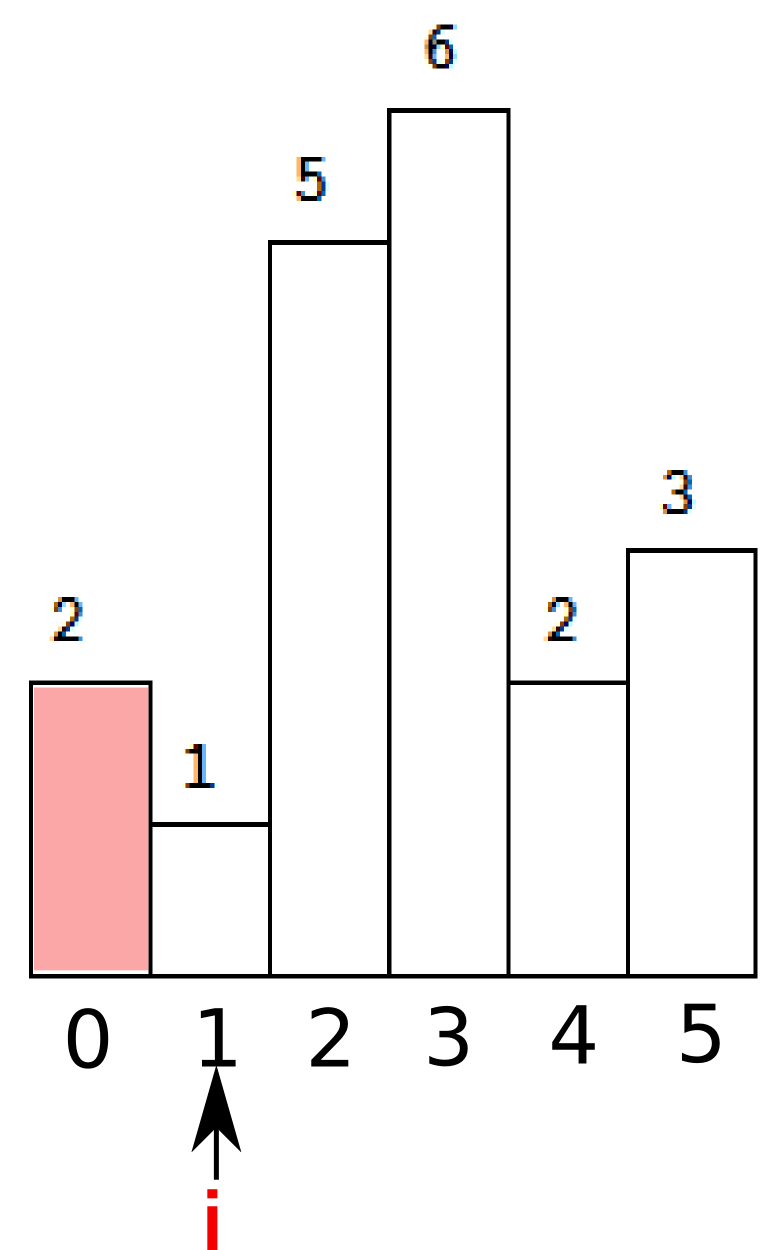
\includegraphics[width=0.5\linewidth]{008401.png}
\end{center}
\begin{CJK}{UTF8}{gbsn}
然后继续,当$i=1$的时候,发现$h[i]$小于了栈内的元素,于是出栈。(由此可以想到,哦,看来stack里面只存放单调递增的索引)
这时候stack为空,所以面积的计算是$h[t] \times i$. $t$是刚刚弹出的stack顶元素。也就是蓝色部分的面积。
\end{CJK}
\begin{center}
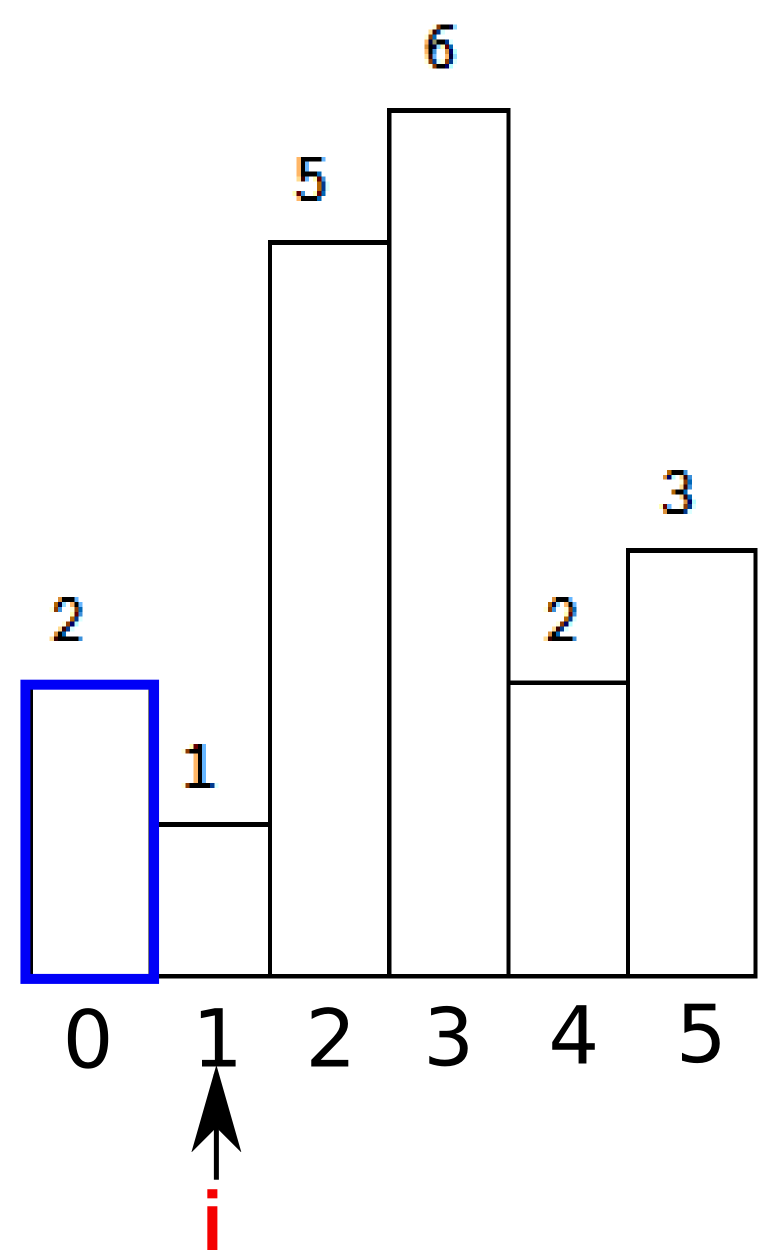
\includegraphics[width=0.5\linewidth]{008402.png}
\end{center}
\begin{CJK}{UTF8}{gbsn}
继续。这时候stack为空了,继续入栈。注意到只要是连续递增的序列,我们都要keep pushing,直到我们遇到了$i=4$,$h[i]=2$小于了栈顶的元素。
\end{CJK}
\begin{center}
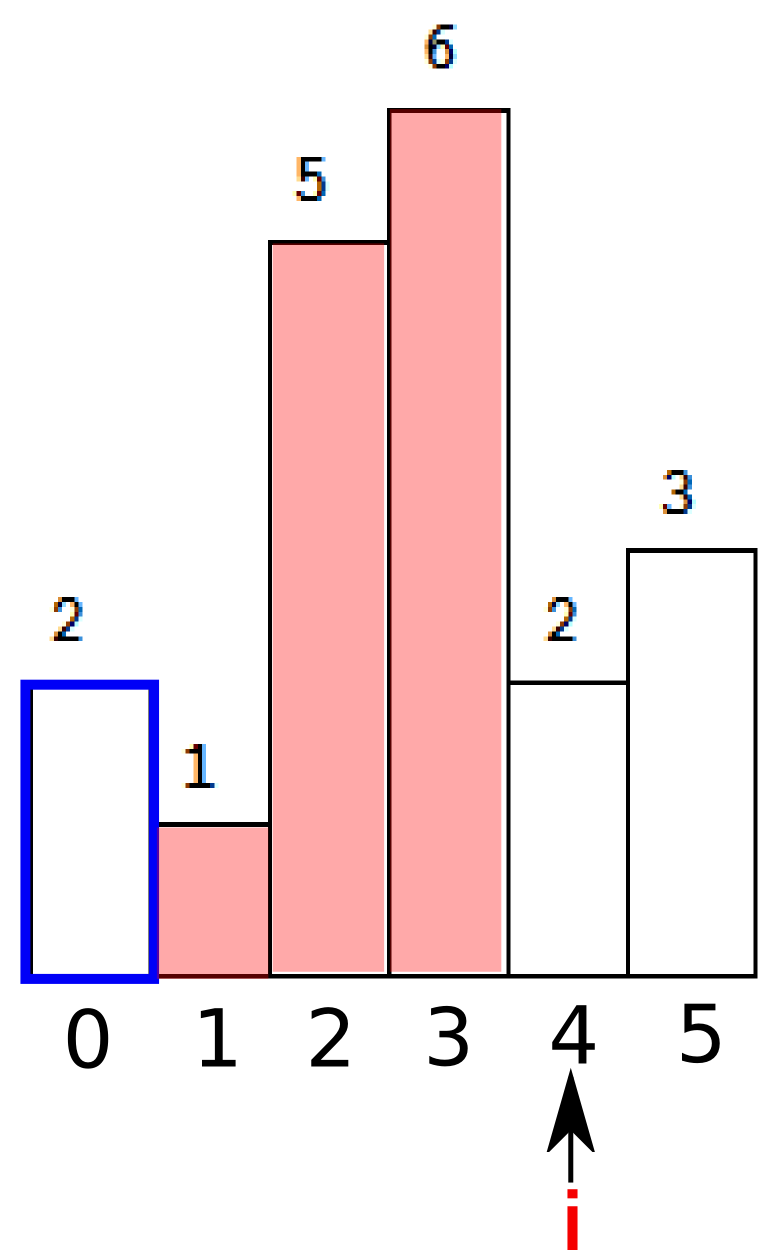
\includegraphics[width=0.5\linewidth]{008403.png}
\end{center}
\begin{CJK}{UTF8}{gbsn}
这时候开始计算矩形面积。首先弹出栈顶元素,$t=3$。即下图绿色部分。
\end{CJK}
\begin{center}
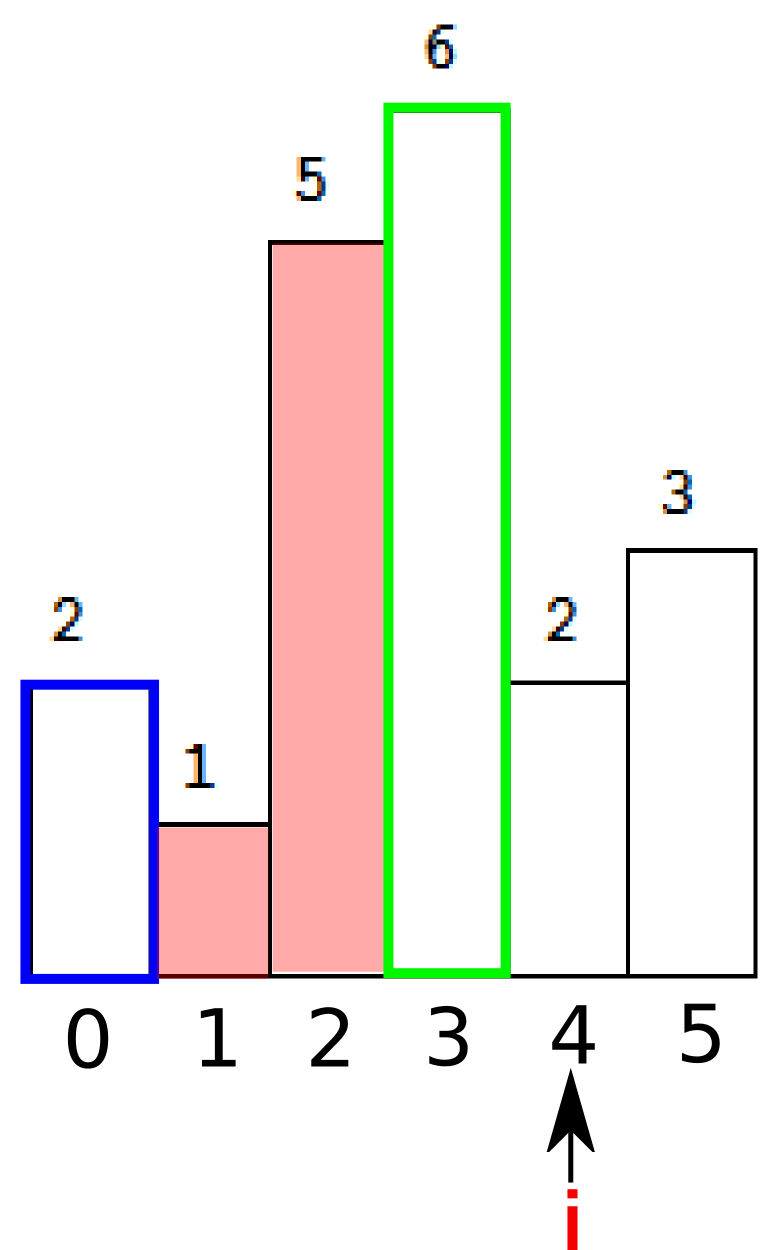
\includegraphics[width=0.5\linewidth]{008404.png}
\end{center}
\begin{CJK}{UTF8}{gbsn}
接下来注意到栈顶的(索引指向的)元素还是大于当前i指向的元素,于是出栈,并继续计算面积,桃红色部分。
\end{CJK}
\begin{center}
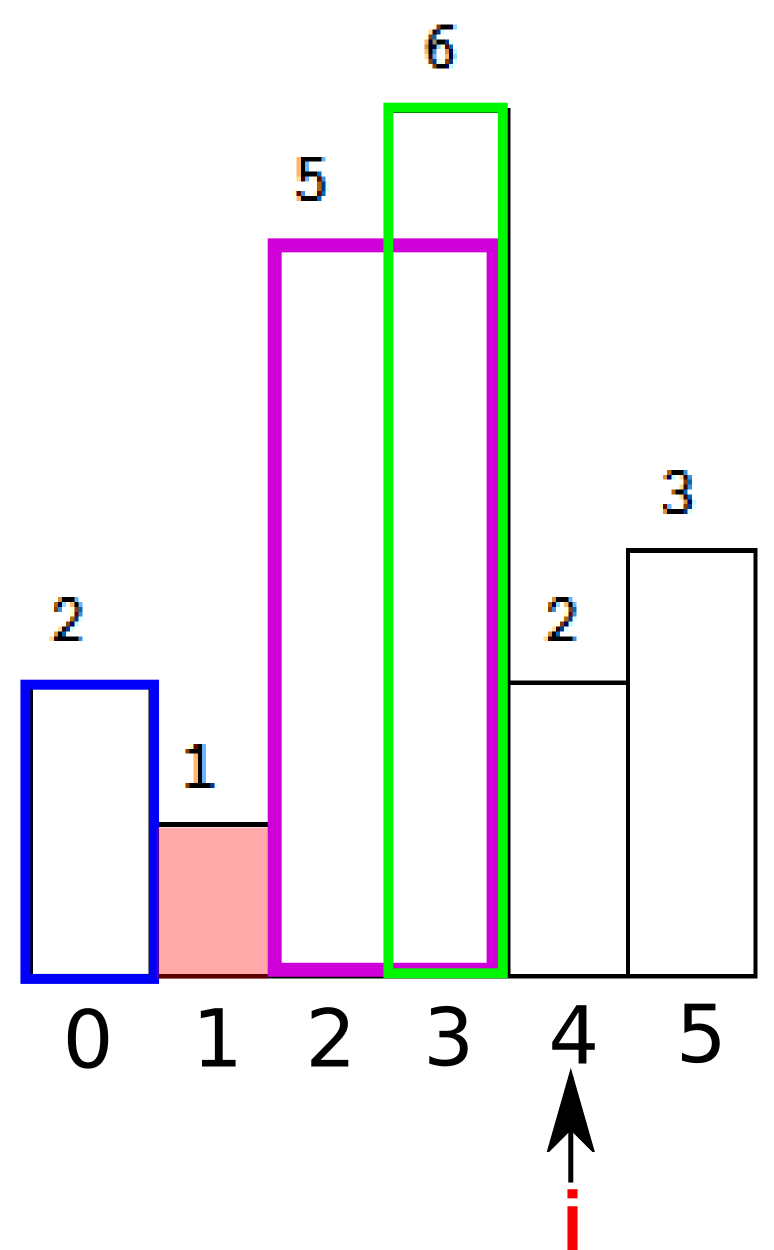
\includegraphics[width=0.5\linewidth]{008405.png}
\end{center}
\begin{CJK}{UTF8}{gbsn}
最后,栈顶的(索引指向的)元素大于了当前$i$指向的元素,循环继续,入栈并推动$i$前进。直到我们再次遇到下降的元素,也就是我们最后人为添加的dummy元素0.
\end{CJK}
\begin{center}
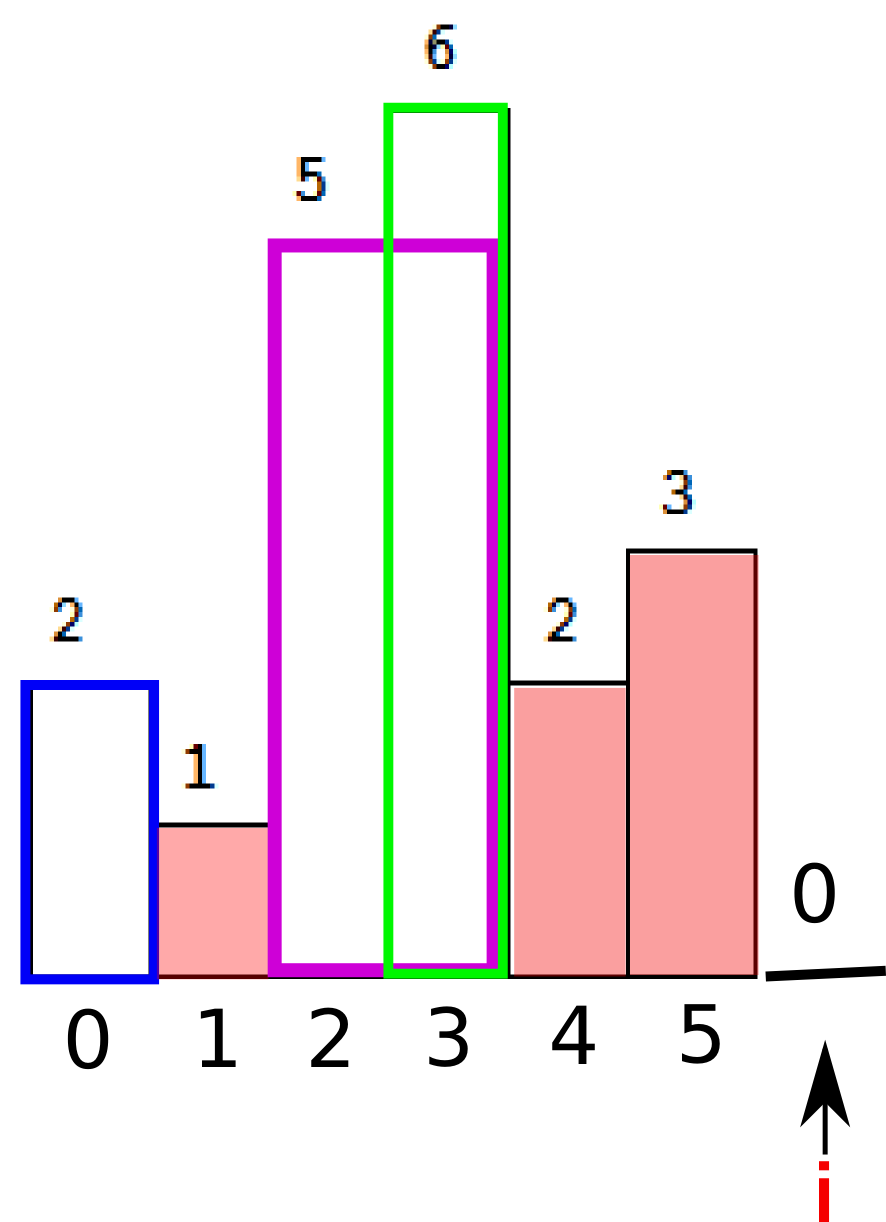
\includegraphics[width=0.5\linewidth]{008406.png}
\end{center}
\begin{CJK}{UTF8}{gbsn}
同理,我们计算栈内的面积。由于当前$i$是最小元素,所以所有的栈内元素都要被弹出并参与面积计算。
\end{CJK}
\begin{center}
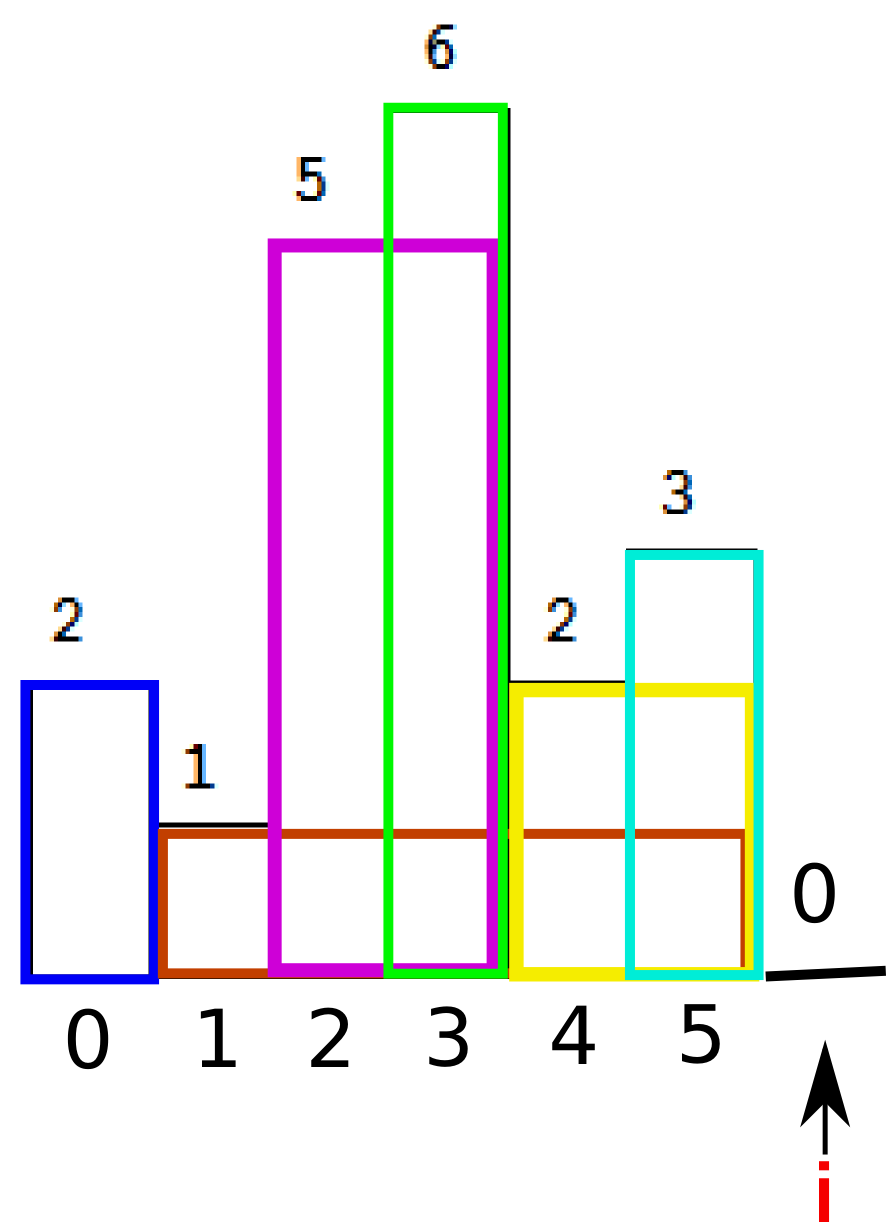
\includegraphics[width=0.5\linewidth]{008407.png}
\end{center}
\begin{CJK}{UTF8}{gbsn}
注意我们在计算面积的时候已经更新过了maxArea。总结下,我们可以看到,stack中总是保持递增的元素的索引,然后当遇到较小的元素后,依次出栈并计算栈中bar能围成的面积,直到栈中元素小于当前元素。
\end{CJK}
\begin{lstlisting}
int largestRectangleArea(vector<int> &height) {
	int res = 0;
	stack<int> s;
	height.push_back(0);
	for (int i = 0; i < height.size(); ++i) {
		if (s.empty() || height[s.top()] < height[i]) s.push(i);
		else {
			int cur = s.top();
			s.pop();
			res = max(res, height[cur] * (s.empty() ? i : (i - s.top() - 1)));
			--i;
		}
	}
	return res;
}
\end{lstlisting}


\section{85}
\begin{CJK}{UTF8}{gbsn}
此题是之前那道的 Largest Rectangle in Histogram 直方图中最大的矩形 的扩展,这道题的二维矩阵每一层向上都可以看做一个直方图,输入矩阵有多少行,就可以形成多少个直方图,对每个直方图都调用 Largest Rectangle in Histogram 直方图中最大的矩形 中的方法,就可以得到最大的矩形面积。那么这道题唯一要做的就是将每一层构成直方图,由于题目限定了输入矩阵的字符只有 \textcolor{red}{0} 和 \textcolor{red}{1} 两种,所以处理起来也相对简单。方法是,对于每一个点,如果是\textcolor{red}{0},则赋0,如果是 \textcolor{red}{1},就赋 之前的height值加上1
\end{CJK}
\begin{lstlisting}
class Solution {
public:
	int maximalRectangle( vector<vector<char> > &matrix ) {
		int res = 0;
		vector<int> height;
		for ( int i = 0; i < matrix.size(); ++i ) {
			height.resize( matrix[i].size() );
			for ( int j = 0; j < matrix[i].size(); ++j ) {
				height[j] = matrix[i][j] == '0' ? 0 : (1 + height[j]);
			}
			res = max( res, largestRectangleArea( height ) );
		}
		return res;
	}
	int largestRectangleArea( vector<int> &height ) {
		int res = 0;
		stack<int> s;
		height.push_back( 0 );
		for ( int i = 0; i < height.size(); ++i ) {
			if ( s.empty() || height[s.top()] <= height[i] ) s.push( i );
			else {
				int tmp = s.top();
				s.pop();
				res = max( res, height[tmp] * (s.empty() ? i : (i - s.top() - 1)) );
				--i;
			}
		}
		return res;
	}
};
\end{lstlisting}
\begin{CJK}{UTF8}{gbsn}
下面这种方法的思路很巧妙,height数组和上面一样,这里的left数组表示左边界是1的位置,right数组表示右边界是1的位置,那么对于任意一行的第j个位置,矩形为(right[j] - left[j]) $\times$ height[j],我们举个例子来说明,比如给定矩阵为:
\end{CJK}
\[
\begin{bmatrix}
1 & 1 & 0 & 0 & 1 \\
0 & 1 & 0 & 0 & 1 \\
0 & 0 & 1 & 1 & 1 \\
0 & 0 & 1 & 1 & 1 \\
0 & 0 & 0 & 0 & 1
\end{bmatrix}
\]
\begin{center}
row = 0:
\begin{tabular}{l*{5}{c}}
h: & 1 & 1 & 0 & 0 & 1 \\
l: & 0 & 0 & 0 & 0 & 4 \\
r: & 2 & 2 & 5 & 5 & 5 
\end{tabular}
\end{center}
\begin{center}
row = 1:
\begin{tabular}{l*{5}{c}}
h: & 1 & 1 & 0 & 0 & 1 \\
l: & 0 & 0 & 0 & 0 & 4 \\
r: & 2 & 2 & 5 & 5 & 5 
\end{tabular}
\end{center}
\begin{center}
row = 2:
\begin{tabular}{l*{5}{c}}
h: & 0 & 0 & 1 & 1 & 3 \\
l: & 0 & 0 & 2 & 2 & 4 \\
r: & 5 & 5 & 5 & 5 & 5 
\end{tabular}
\end{center}
\begin{center}
row = 3:
\begin{tabular}{l*{5}{c}}
h: & 0 & 0 & 2 & 2 & 4 \\
l: & 0 & 0 & 2 & 2 & 4 \\
r: & 5 & 5 & 5 & 5 & 5 
\end{tabular}
\end{center}
\begin{center}
row = 4:
\begin{tabular}{l*{5}{c}}
h: & 0 & 0 & 0 & 0 & 5 \\
l: & 0 & 0 & 0 & 0 & 4 \\
r: & 5 & 5 & 5 & 5 & 5 
\end{tabular}
\end{center}
\begin{lstlisting}
int maximalRectangle( vector<vector<char>>& matrix ) {
	if ( matrix.empty() || matrix[0].empty() ) return 0;
	int res = 0, m = matrix.size(), n = matrix[0].size();
	vector<int> height( n, 0 ), left( n, 0 ), right( n, n );
	for ( int i = 0; i < m; ++i ) {
		int cur_left = 0, cur_right = n;
		for ( int j = 0; j < n; ++j ) {
			if ( matrix[i][j] == '1' ) ++height[j];
			else height[j] = 0;
		}
		for ( int j = 0; j < n; ++j ) {
			if ( matrix[i][j] == '1' ) left[j] = max( left[j], cur_left );
			else { left[j] = 0; cur_left = j + 1; }
		}
		for ( int j = n - 1; j >= 0; --j ) {
			if ( matrix[i][j] == '1' ) right[j] = min( right[j], cur_right );
			else { right[j] = n; cur_right = j; }
		}
		for ( int j = 0; j < n; ++j ) {
			res = max( res, (right[j] - left[j]) * height[j] );
		}
	}
	return res;
}
\end{lstlisting}

\section{86}
\begin{CJK}{UTF8}{gbsn}
这道题要求我们划分链表,把所有小于给定值的节点都移到前面,大于该值的节点顺序不变,相当于一个局部排序的问题。那么可以想到的一种解法是首先找到第一个大于或等于给定值的节点,用题目中给的例子来说就是先找到4,然后再找小于3的值,每找到一个就将其取出置于4之前即可
\end{CJK}
\begin{lstlisting}
ListNode *partition( ListNode *head, int x ) {
	ListNode *dummy = new ListNode( -1 );
	dummy->next = head;
	ListNode *pre = dummy, *cur = head;;
	while ( pre->next && pre->next->val < x ) pre = pre->next;
	cur = pre;
	while ( cur->next ) {
		if ( cur->next->val < x ) {
			ListNode *tmp = cur->next;
			cur->next = tmp->next;
			tmp->next = pre->next;
			pre->next = tmp;
			pre = pre->next;
		}
		else {
			cur = cur->next;
		}
	}
	return dummy->next;
}
\end{lstlisting}
\begin{CJK}{UTF8}{gbsn}
此题还有一种解法,就是将所有小于给定值的节点取出组成一个新的链表,此时原链表中剩余的节点的值都大于或等于给定值,只要将原链表直接接在新链表后即可
\end{CJK}
\begin{lstlisting}
ListNode *partition( ListNode *head, int x ) {
	if ( !head ) return head;
	ListNode *dummy = new ListNode( -1 );
	ListNode *newDummy = new ListNode( -1 );
	dummy->next = head;
	ListNode *cur = dummy, *p = newDummy;
	while ( cur->next ) {
		if ( cur->next->val < x ) {
			p->next = cur->next;
			p = p->next;
			cur->next = cur->next->next;
			p->next = NULL;
		}
		else {
			cur = cur->next;
		}
	}
	p->next = dummy->next;
	return newDummy->next;
}
\end{lstlisting}

\section{87}
\begin{CJK}{UTF8}{gbsn}
这道题定义了一种爬行字符串,就是说假如把一个字符串当做一个二叉树的根,然后它的非空子字符串是它的子节点,然后交换某个子字符串的两个子节点,重新爬行回去形成一个新的字符串,这个新字符串和原来的字符串互为爬行字符串。这道题可以用递归Recursion或是动态规划Dynamic Programming来做,我们先来看递归的解法,
\par
就是s1和s2是scramble的话,那么必然存在一个在s1上的长度l1,将s1分成s11和s12两段,同样有s21和s22.
\par
那么要么s11和s21是scramble的并且s12和s22是scramble的;要么s11和s22是scramble的并且s12和s21是scramble的。
\par
就拿题目中的例子 rgeat 和 great 来说,rgeat 可分成 rg 和 eat 两段, great 可分成 gr 和 eat 两段,rg 和 gr 是scrambled的, eat 和 eat 当然是scrambled。
\end{CJK}
\begin{lstlisting}
bool isScramble( string s1, string s2 ) {
	if ( s1.size() != s2.size() ) return false;
	if ( s1 == s2 ) return true;
	string str1 = s1, str2 = s2;
	sort( str1.begin(), str1.end() );
	sort( str2.begin(), str2.end() );
	if ( str1 != str2 ) return false;
	for ( int i = 1; i < s1.size(); ++i ) {
		string s11 = s1.substr( 0, i );
		string s12 = s1.substr( i );
		string s21 = s2.substr( 0, i );
		string s22 = s2.substr( i );
		if ( isScramble( s11, s21 ) && isScramble( s12, s22 ) ) return true;
		s21 = s2.substr( s1.size() - i );
		s22 = s2.substr( 0, s1.size() - i );
		if ( isScramble( s11, s21 ) && isScramble( s12, s22 ) ) return true;
	}
	return false;
}
\end{lstlisting}
\begin{CJK}{UTF8}{gbsn}
当然,这道题也可以用动态规划Dynamic Programming,根据以往的经验来说,根字符串有关的题十有八九可以用DP来做,那么难点就在于如何找出递推公式。这其实是一道三维动态规划的题目,我们提出维护量res[i][j][n],其中i是s1的起始字符,j是s2的起始字符,而n是当前的字符串长度,res[i][j][len]表示的是以i和j分别为s1和s2起点的长度为len的字符串是不是互为scramble。
\par
有了维护量我们接下来看看递推式,也就是怎么根据历史信息来得到res[i][j][len]。判断这个是不是满足,其实我们首先是把当前s1[i,i+len-1]字符串劈一刀分成两部分,然后分两种情况:第一种是左边和s2[j,j+len-1]左边部分是不是scramble,以及右边和s2[j,j+len-1]右边部分是不是scramble;第二种情况是左边和s2[j,j+len-1]右边部分是不是scramble,以及右边和s2[j,j+len-1]左边部分是不是scramble。如果以上两种情况有一种成立,说明s1[i,i+len-1]和s2[j,j+len-1]是scramble的。而对于判断这些左右部分是不是scramble我们是有历史信息的,因为长度小于n的所有情况我们都在前面求解过了(也就是长度是最外层循环)。
上面说的是劈一刀的情况,对于s1[i,i+len-1]我们有len-1种劈法,在这些劈法中只要有一种成立,那么两个串就是scramble的。
总结起来递推式是res[i][j][len] = || (res[i][j][k]\&\&res[i+k][j+k][len$-$k] || res[i][j+len$-$k][k]\&\&res[i+k][j][len$-$k]) 对于所有1\textless=k\textless len,也就是对于所有len$-$1种劈法的结果求或运算。因为信息都是计算过的,对于每种劈法只需要常量操作即可完成,因此求解递推式是需要$O(len)$(因为len$-$1种劈法)。
如此总时间复杂度因为是三维动态规划,需要三层循环,加上每一步需要线行时间求解递推式,所以是$O(n^4)$。虽然已经比较高了,但是至少不是指数量级的,动态规划还是有很大优势的,空间复杂度是$O(n^3)$
\end{CJK}
\begin{lstlisting}
bool isScramble( string s1, string s2 ) {
	if ( s1.size() != s2.size() ) return false;
	if ( s1 == s2 ) return true;
	int n = s1.size();
	vector<vector<vector<bool> > > dp( n, vector<vector<bool> >( n, vector<bool>( n + 1, false ) ) );
	for ( int i = 0; i < n; ++i ) {
		for ( int j = 0; j < n; ++j ) {
			dp[i][j][1] = s1[i] == s2[j];
		}
	}
	for ( int len = 2; len <= n; ++len ) {
		for ( int i = 0; i <= n - len; ++i ) {
			for ( int j = 0; j <= n - len; ++j ) {
				for ( int k = 1; k < len; ++k ) {
					if ( (dp[i][j][k] && dp[i + k][j + k][len - k]) || (dp[i + k][j][len - k] && dp[i][j + len - k][k]) ) {
						dp[i][j][len] = true;
					}
				}
			}
		}
	}
	return dp[0][0][n];
}
};
\end{lstlisting}
\begin{CJK}{UTF8}{gbsn}
上面的代码的实现过程如下,首先按单个字符比较,判断它们之间是否是scrambled的。在更新第二个表中第一个值(gr和rg是否为scrambled的)时,比较了第一个表中的两种构成,一种是 g与r, r与g,另一种是 g与g, r与r,其中后者是真,只要其中一个为真,则将该值赋真。其实这个原理和之前递归的原理很像,在判断某两个字符串是否为scrambled时,比较它们所有可能的拆分方法的子字符串是否是scrambled的,只要有一个种拆分方法为真,则比较的两个字符串一定是scrambled的。比较 rge 和 gre 的实现过程如下所示:
\end{CJK}
\par
\begin{tabular}{l*{3}{c}}
  & r & g & e \\
g & \ding{55} & \ding{51} & \ding{55} \\
r & \ding{51} & \ding{55} & \ding{55} \\
e & \ding{55} & \ding{55} & \ding{51} \\
\end{tabular}
\par
\begin{tabular}{l*{2}{c}}
&  rg & ge \\
gr & \ding{51} & \ding{55} \\
re & \ding{55} & \ding{55} \\
\end{tabular}
\par
\begin{tabular}{lc}
&  rge \\
gre & \ding{51} \\
\end{tabular}
\par
\begin{CJK}{UTF8}{gbsn}
DP的另一种写法: dp[i][j][k] 代表了s1从i开始,s2从j开始,长度为k的两个substring是否为scramble
string。有三种情况需要考虑:
\begin{enumerate}
\item 如果两个substring相等的话,则为true
\item 如果两个substring中间某一个点,左边的substrings为scramble string,同时右边的substrings也为scramble string,则为true
\item 如果两个substring中间某一个点,s1左边的substring和s2右边的substring为scramble string, 同时s1右边substring和s2左边的substring也为scramble string,则为true.
\end{enumerate}
\end{CJK}
\begin{lstlisting}
bool isScramble( string s1, string s2 ) {
	if ( s1.size() != s2.size() ) return false;
	if ( s1 == s2 ) return true;
	int n = s1.size();
	vector<vector<vector<bool> > > dp( n, vector<vector<bool> >( n, vector<bool>( n + 1, false ) ) );
	for ( int i = n - 1; i >= 0; --i ) {
		for ( int j = n - 1; j >= 0; --j ) {
			for ( int k = 1; k <= n - max( i, j ); ++k ) {
				if ( s1.substr( i, k ) == s2.substr( j, k ) ) {
					dp[i][j][k] = true;
				}
				else {
					for ( int t = 1; t < k; ++t ) {
						if ( (dp[i][j][t] && dp[i + t][j + t][k - t]) || (dp[i][j + k - t][t] && dp[i + t][j][k - t]) ) {
							dp[i][j][k] = true;
							break;
						}
					}
				}
			}
		}
	}
	return dp[0][0][n];
}
\end{lstlisting}
\begin{CJK}{UTF8}{gbsn}
下面这种解法和第一个解法思路相同,只不过没有用排序算法,而是采用了类似于求异构词的方法,用一个数组来保存每个字母出现的次数,后面判断Scramble字符串的方法和之前的没有区别:
\end{CJK}
\begin{lstlisting}
bool isScramble( string s1, string s2 ) {
	if ( s1 == s2 ) return true;
	if ( s1.size() != s2.size() ) return false;
	int n = s1.size(), m[26] = { 0 };
	for ( int i = 0; i < n; ++i ) {
		++m[s1[i] - 'a'];
		--m[s2[i] - 'a'];
	}
	for ( int i = 0; i < 26; ++i ) {
		if ( m[i] != 0 ) return false;
	}
	for ( int i = 1; i < n; ++i ) {
		if ( (isScramble( s1.substr( 0, i ), s2.substr( 0, i ) ) && isScramble( s1.substr( i ), s2.substr( i ) )) || (isScramble( s1.substr( 0, i ), s2.substr( n - i ) ) && isScramble( s1.substr( i ), s2.substr( 0, n - i ) )) ) {
			return true;
		}
	}
	return false;
}
\end{lstlisting}


\section{88}
\begin{CJK}{UTF8}{gbsn}
混合插入有序数组,由于两个数组都是有序的,所有只要按顺序比较大小即可。最先想到的方法是建立一个$m+n$大小的新数组,然后逐个从A和B数组中取出元素比较,把较小的加入新数组,然后在考虑A数组有剩余和B数组有剩余的两种情况,最后在把新数组的元素重新赋值到A数组中即可
\end{CJK}
\begin{lstlisting}
void merge( int A[], int m, int B[], int n ) {
	if ( m <= 0 && n <= 0 ) return;
	int a = 0, b = 0;
	int C[m + n];
	for ( int i = 0; i < m + n; ++i ) {
		if ( a < m && b < n ) {
			if ( A[a] < B[b] ) {
				C[i] = A[a];
				++a;
			}
			else {
				C[i] = B[b];
				++b;
			}
		}
		else if ( a < m && b >= n ) {
			C[i] = A[a];
			++a;
		}
		else if ( a >= m && b < n ) {
			C[i] = B[b];
			++b;
		}
		else return;
	}
	for ( int i = 0; i < m + n; ++i ) A[i] = C[i];
}
\end{lstlisting}
\begin{CJK}{UTF8}{gbsn}
这样固然没错,但是还有更简洁的方法,而且不用申请新变量。算法思想是:由于合并后A数组的大小必定是$m+n$,所以从最后面开始往前赋值,先比较A和B中最后一个元素的大小,把较大的那个插入到$m+n-1$的位置上,再依次向前推。如果A中所有的元素都比B小,那么前m个还是A原来的内容,没有改变。如果A中的数组比B大的,当A循环完了,B中还有元素没加入A,直接用个循环把B中所有的元素覆盖到A剩下的位置。
\end{CJK}
\begin{lstlisting}
void merge( int A[], int m, int B[], int n ) {
	int count = m + n - 1;
	--m; --n;
	while ( m >= 0 && n >= 0 ) A[count--] = A[m] > B[n] ? A[m--] : B[n--];
	while ( n >= 0 ) A[count--] = B[n--];
}
\end{lstlisting}
\end{document}